\documentclass[11pt,a4paper]{article}
\usepackage[utf8]{inputenc}
\usepackage{amsmath}
\usepackage{amsfonts}
\usepackage{amssymb}
\usepackage{graphicx}
\usepackage[top=3cm, bottom=3cm, left=2cm , right=2cm]{geometry}
\begin{document}
\author{Iserentant Merlin - Momin Charles}
\title{Rapport projet 2: Factorisation de nombres}
\maketitle

Ce rapport comporte une analyse détaillée de l'architecture et du fonctionnement de notre programme ainsi qu'un analyse paramétrique des perfomances de ce dernier. 

\section*{Architecture globale du programme}
Notre programme est divisé en 4 phases principales distinctes:

\begin{itemize}
\item{Chargement des nombres: cette phase se compose d'une analyse des paramètres du programme suivie d'une phase de chargement des nombre à proprement parlée.)}
\item{Factorisation des nombres: comme son nom l'indique, cette étape sert à factoriser les nombres obtenue grâce à la phase précédente en facteur premier.}
\item{Traitement des facteurs premiers: chaque facteur produit par la factorisation et traité. Un compte de chacun des facteurs est tenu. Les nombres premiers manquants sont également calculés}
\item{Analyse des résultats: le facteur unique trouvé est cherché parmis les différents compteurs. Si plusieurs facteurs unique sont trouvés, une erreur est envoyée.}
\end{itemize}

Les trois premières étapes se déroulent de manière simultanée grâce à l'utilisation de threads selon un double schéma de producteur/consommateur. Les chargements de nombres se font à raison d'un thread par type d'entrée de nombre. Plus précisément, chacun de ces threads itère sur un tableau contenant les différents noms de fichier ou adresses URL. Il y a donc trois threads de chargement de nombre.  La taille du buffer pour le premier schéma est de N et celle du deuxième buffer est de N+1. N places sont réservées pour les threads qui incremétentent les comptes et la dernière l'est pour le thread de calcul. Ce choix n'est pas anodin, en effet il permet à N threads de factorisations fonctionner en simultanée. L'incrémentation des compteurs se fait grâce à CHECK ICI LE NOMBRE DE THREADS de thread parcourant le second buffer qui met à jours les comptes des différents facteurs premiers trouvés et un thread qui calcul les nombres premiers manquant lorsque c'est nécessaire.
Le thread qui calcul les nombres premiers est unique car le programme ne doit calculer qu'un nombre premier à la fois. 
Une fois ces étapes faites, le programme principale analyse les compteurs obtenus(4eme étape).

\section*{Mécanisme de synchronisation}
Les différents échanges de données entre threads se font grâce à deux schémas de producteur/consommateur 

\begin{itemize}
\item{Premier schéma: [Producteur]=Threads de chargement de nombres $\Rightarrow$ sortie:nombres sur 64bits; [Consommateurs]=Threads de factorisation}
\item{Second schéma: [Producteur]=Threads de factorisation $\Rightarrow$ sortie:nombres premiers; [Consommateurs1]=Threads qui gèrent les comptes des facteurs premiers, [Consammateur2]=Threads de calcul de nombre premiers}
\end{itemize}

L'implémentation de ces schémas est réalisée grâce à l'utilisation de sémaphores, permettant ainsi l'accès aux buffers.

Les buffers sont des tableaux de taille N. Leurs accès est protégé en plus des sémaphores par des mutex qui évitent tout problème de synchronisation entre threads lors de l'écriture de données.

\section*{Structure de données}
Les structures utilisées sont les suivantes:

\begin{itemize}
\item{Premier schéma de producteur/consommateur: tableau de nombres de dimension [2xN]. La première dimension contient le nombre et la deuxième une référence vers le fichier d'origine}
\item{Second schéma de producteur/consommateur: tableau de nombres de dimension [2xN]. La première dimension contient le nombre et la seconde une référence vers le fichier d'origine. Et un pointeur vers un nombre qui contient le dernier nombre premier lorsqu'il faut calculer le nombre premier suivant.}
\item{Structure de nombre premier: structure contenant un nombre premier, le compte de celui-ci ainsi qu'une référence vers le fichier dans lequel la dernière itération de ce nombre a été trouvée.}
\item{Liste chainée de structure de nombre premier: Liste des nombres premiers et leurs comptes. Elle est mise à jour si nécessaire.}
\end{itemize}


\section*{Algorithmes principaux}
 \subsection*{Algorithme 1: génération de nombres premier}
 
Pour tester si un nombre est premier, notre programme teste s'il est divisible par tous les nombres premiers inférieurs à sa racine carré (ceux-ci sont déjà calculés et stockés dans la liste chainée). Si ce n'est pas le cas, il s'agit bien d'un nombre premier. 
 
 
 \subsection*{Algorithme 2: Factorisation en produit de nombre premier}   
 
 On procède par itération. Notre programme test le nombre afin de voir si il est divisible par le plus petit nombre premier (2). Si c'est le cas, on considère que ce nombre premier est facteur et on réitère le test sur le résultat de la division ainsi obtenu. Si le test venait à échouer, le test de division s'effectue avec le nombre premier suivant (si la liste chainée n'indique pas de nombre premier suivant, celui-ci est calculé à l'aide de l'algorithme 1 et rajouté à la liste chainée). Les tests de division s'arrête lorsque le nombre est devenu égale à l'unité.
 
\section*{Analyses de performances}

Durant l'implémentation du projet, nous avons posé différents choix afin d'optimiser les performances temporelles de notre programme. Nous allons analyser ci-après les plus importantes d'entre elles qui nous semble importante à l'aide de graphiques réalisés sur matlab en fonction de résultats expérimentaux.

Les premiers tests de performance ont été réalisés sur les machines en salle intel. Deux types de tests ont été effectués: varitation du nombre $N$ de threads de factorisation et variation du nombre de threads consommateurs du second buffer. Les résultats obtenus sont présentées aux figures 1 et 2.

\begin{figure}[ht!]
 \centering
 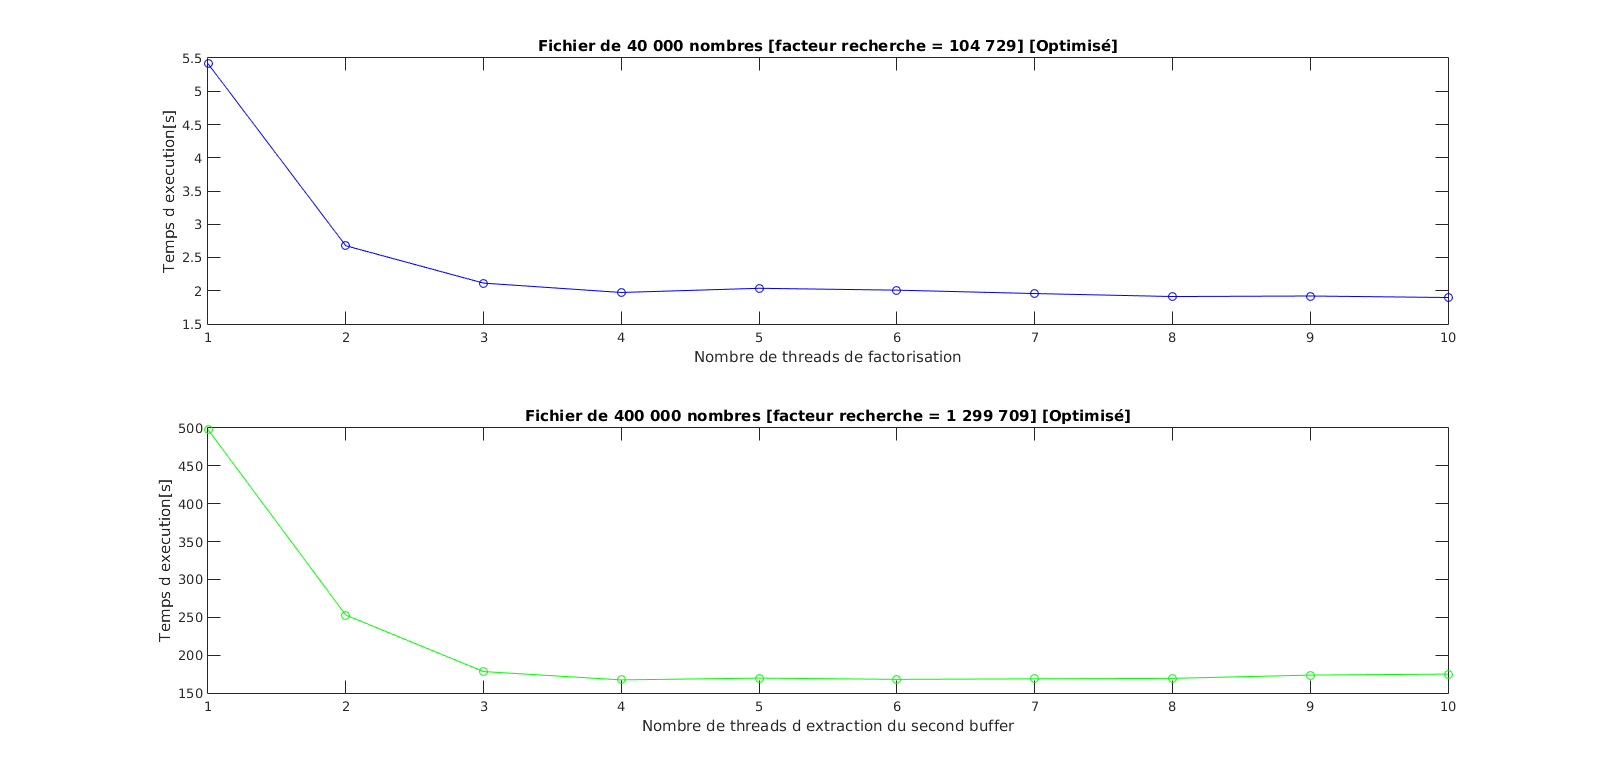
\includegraphics[scale=0.4]{NanaOpt.png}
 \caption{Variation du nombre de threads $N$}
 \label{schemefig1}
\end{figure}

\begin{figure}[ht!]
 \centering
 \begin{center}
 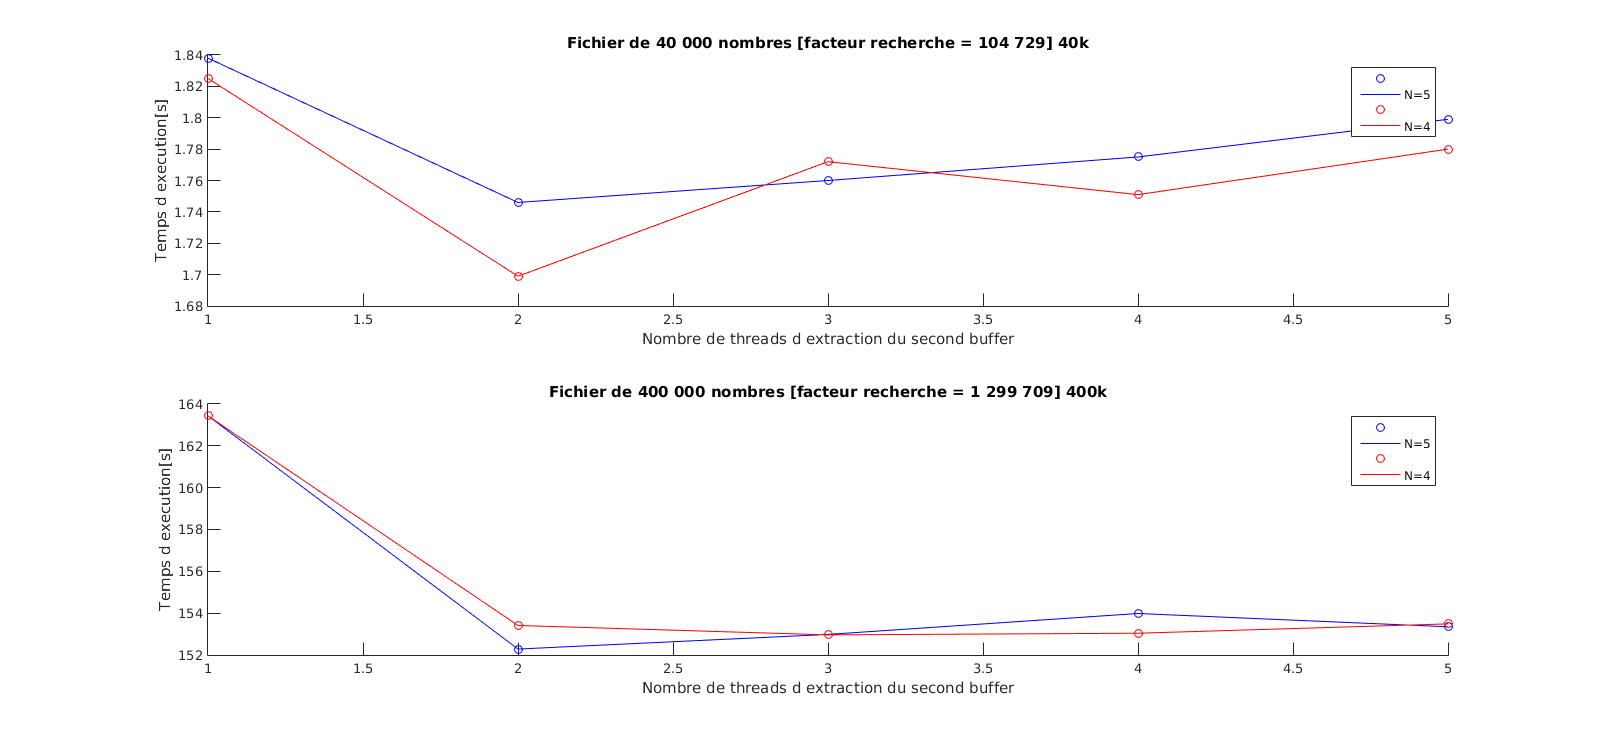
\includegraphics[scale=0.4]{kanaOpt.png} 
 \end{center}
 \caption{Variation du nombre de threads consommateurs}
 \label{scheme1}
\end{figure}

L'analyse des résultats montre l'existence d'un nombre de thread optimale pour le traitement d'un fichier de taille définie, contenant des nombres de taille définie eux aussi. Dans le cas présent, ce nombre tourne au alentours de 4. La perte de performance provoquée par un nombre supérieur au nombre optimal vient de l'utilisation de mécanisme de synchronisation. Des threads présents en trop grand nombre ont plus de chance de se voir refuser l'accès à leurs section critique. En effet, les différents accès aux données nécessaires sont plus souvent déjà bloqués par un autre thread.

De plus, la performance est liée au nombre de processeur utilisés par la machine. L'utilitaire "$Monitor$" du Linux indique que les machines de la salle Intel possèdent 4 CPUs actif. Afin de montrer l'importance de ce facteur dans les performance de programme, les résultats obtenus dans les même condition d'exécution sur une machine utilisant 8 CPUs sont montrés aux figures 3 et 4.

\begin{figure}[ht!]
 \centering
 %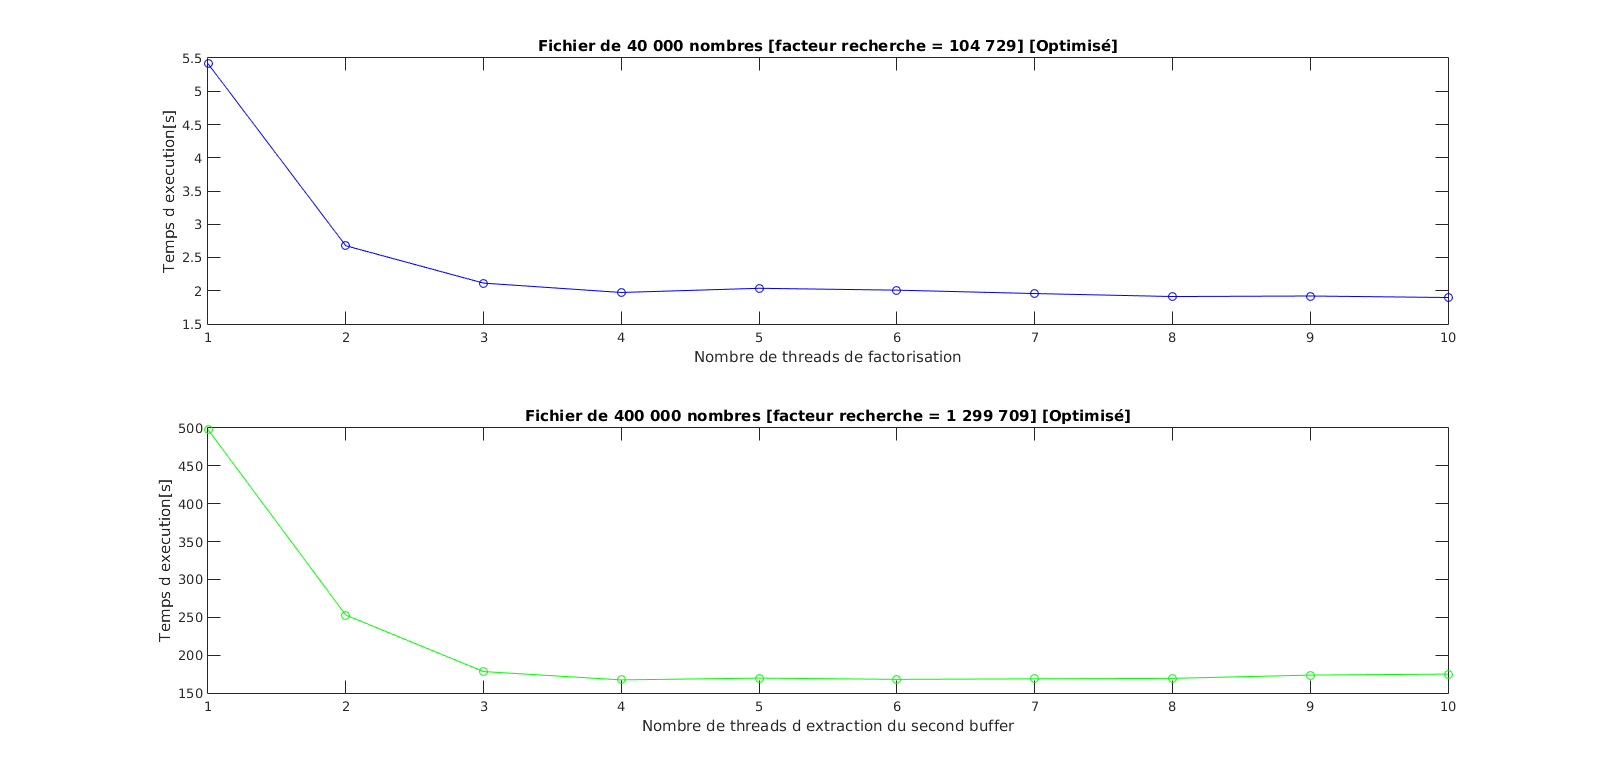
\includegraphics[scale=0.4]{NanaOpt.png}
 \caption{Variation du nombre de threads $N$}
 \label{schemefig1}
\end{figure}

\begin{figure}[ht!]
 \centering
 \begin{center}
 %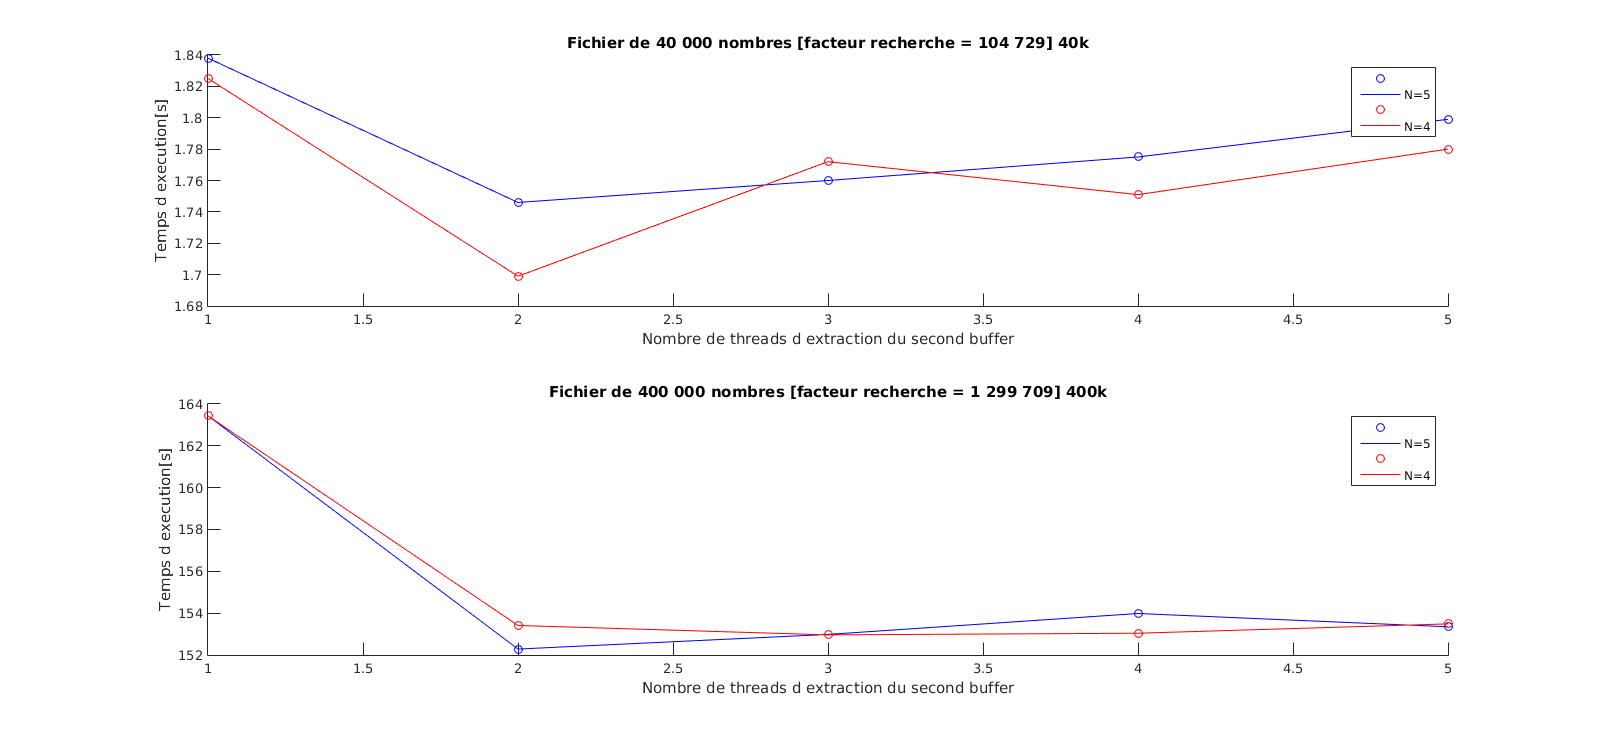
\includegraphics[scale=0.4]{kanaOpt.png} 
 \end{center}
 \caption{Variation du nombre de threads consommateurs}
 \label{scheme1}
\end{figure}

On observe que les graphes des figures 3 et 4 sont de même type que ceux des figures 1 et 2. Un décalage du nombre de thread optimal est cependant observable. Une piste possible d'explication est la suivante: vu le grand nombre de threads utilisés, la machine ne peut pas tous les executer en temps que thread physique. Beaucoup seront donc interrompus en cours d'éxecution afin de permettre à chacun des threads de s'exécuter. Pour le peu qu'un de ces thread ne s'interrompe dans sa section critique, il bloque alors l'accès au différentes ressources protégées par des méchanisme de synchronisation. Les autres threads sont alors à leurs tour bloqués, se qui provoque une perte de temps non-voulue. Le nombre de threads physiques possibles étant défini par le nombre de CPUs, une machine en disposant de plus verra son nombre de thread optimal augmenté.
\end{document}
